\clearpage
\subsection{Compact boson, large intervals}
\label{sec:pair-large_boson}
\begin{figure}[!htbp]\centering
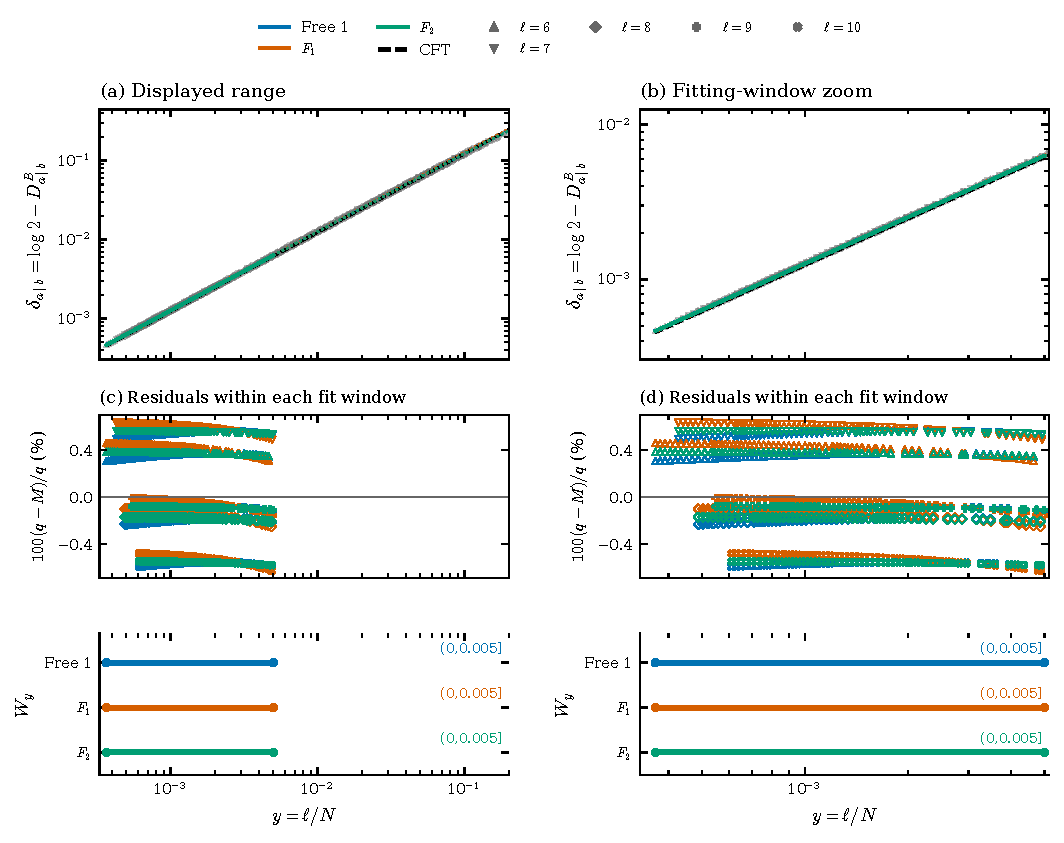
\includegraphics[width=.94\linewidth]{../figs/pair_large_boson_00_ss.pdf}\par\smallskip
\begingroup\scriptsize\setlength{\tabcolsep}{4pt}
\begin{tabular}{lllrrrrr}\toprule
Set & Model & $W_z$ & $m$ & $c_0$ & $r^{(0)}$ & $c_1$ & $r^{(1)}$\\\midrule
Both & Free 1 & $(0,0.005]$ & 317 & 1.2561 & 0.9992554 & --- & ---\\
Both & $F_1$ & $(0,0.005]$ & 317 & 1.2616 & 1 & --- & ---\\
Both & $F_2$ & $(0,0.005]$ & 317 & 1.2627 & 1 & -0.33376 & 2\\
\midrule
Both & CFT & --- & --- & 1.2337 & 1 & --- & ---\\
\bottomrule\end{tabular}
\endgroup
\caption{Compact boson, large intervals, $00\mid ss$, at $p=1/2$, $\ell=6,\ldots,10$, and the complete size grid in Eq.~\eqref{eq:extended-grid}. Here $z=y$ and $q=\delta=\log2-D^B$. Left: all computed data through $z=0.20$; right: a zoom into the common fitting window. Both columns show the same Free 1, $F_1$, and $F_2$ fits. All six directions of this CFT and interval type use the same window. Gray markers denote the data. Colored solid segments lie inside each model\textquotesingle s fitting interval; dotted segments are extrapolations. Black dashed is the analytical CFT leading deficit. The observable axes are logarithmic and span the measured data; nonpositive predictions cannot appear there and out-of-range extrapolations leave the panel. Residual ordinates are linear and show $100(q-M)/q$ only on each model\textquotesingle s fitted observations. Bars give the exact fitting intervals. The parameter block follows Eq.~\eqref{eq:fit}, with $c_0,c_1$ multiplying $z^{r^{(0)}},z^{r^{(1)}}$; all coefficients include powers of $\pi$. A dash means an absent fitted term, or no fitting window for CFT. Values shown are rounded; curves use full precision.}
\label{fig:pair-large_boson-00-ss}
\end{figure}
\begin{figure}[!htbp]\centering
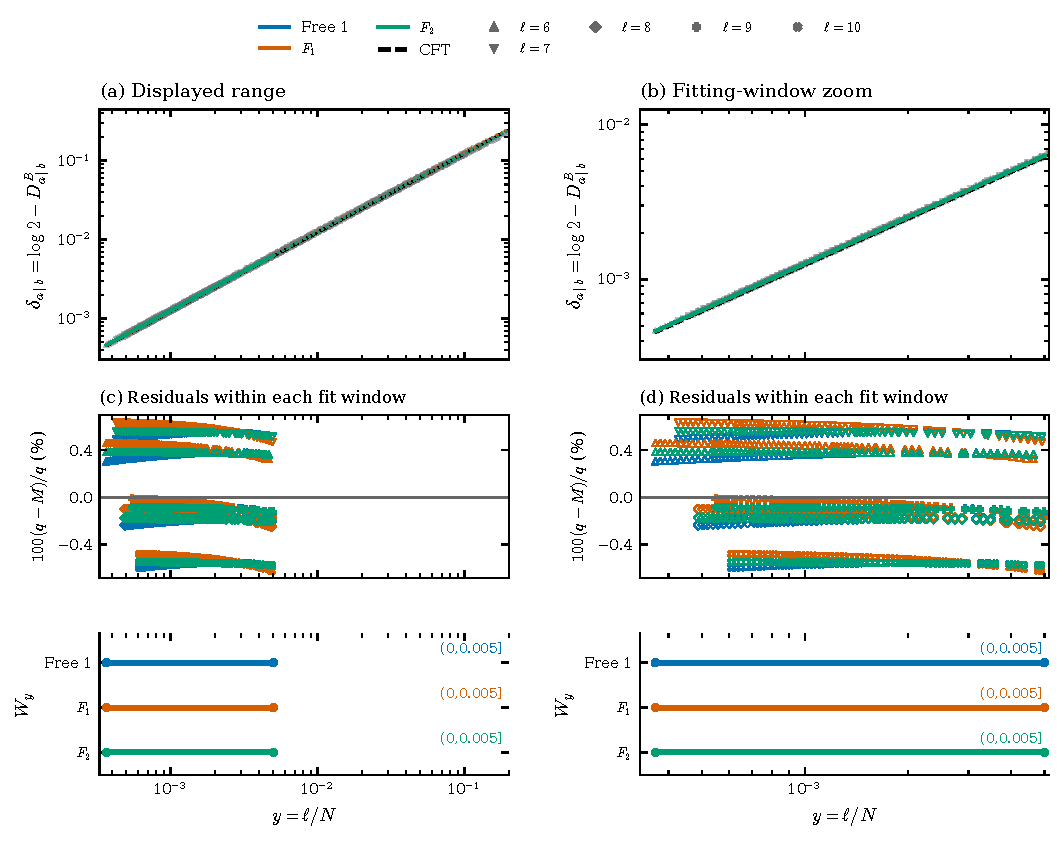
\includegraphics[width=.94\linewidth]{../figs/pair_large_boson_ss_00.pdf}\par\smallskip
\begingroup\scriptsize\setlength{\tabcolsep}{4pt}
\begin{tabular}{lllrrrrr}\toprule
Set & Model & $W_z$ & $m$ & $c_0$ & $r^{(0)}$ & $c_1$ & $r^{(1)}$\\\midrule
Both & Free 1 & $(0,0.005]$ & 317 & 1.256 & 0.9992434 & --- & ---\\
Both & $F_1$ & $(0,0.005]$ & 317 & 1.2616 & 1 & --- & ---\\
Both & $F_2$ & $(0,0.005]$ & 317 & 1.2627 & 1 & -0.34138 & 2\\
\midrule
Both & CFT & --- & --- & 1.2337 & 1 & --- & ---\\
\bottomrule\end{tabular}
\endgroup
\caption{Compact boson, large intervals, $ss\mid 00$, at $p=1/2$, $\ell=6,\ldots,10$, and the complete size grid in Eq.~\eqref{eq:extended-grid}. Here $z=y$ and $q=\delta=\log2-D^B$. Left: all computed data through $z=0.20$; right: a zoom into the common fitting window. Both columns show the same Free 1, $F_1$, and $F_2$ fits. All six directions of this CFT and interval type use the same window. Gray markers denote the data. Colored solid segments lie inside each model\textquotesingle s fitting interval; dotted segments are extrapolations. Black dashed is the analytical CFT leading deficit. The observable axes are logarithmic and span the measured data; nonpositive predictions cannot appear there and out-of-range extrapolations leave the panel. Residual ordinates are linear and show $100(q-M)/q$ only on each model\textquotesingle s fitted observations. Bars give the exact fitting intervals. The parameter block follows Eq.~\eqref{eq:fit}, with $c_0,c_1$ multiplying $z^{r^{(0)}},z^{r^{(1)}}$; all coefficients include powers of $\pi$. A dash means an absent fitted term, or no fitting window for CFT. Values shown are rounded; curves use full precision.}
\label{fig:pair-large_boson-ss-00}
\end{figure}
\begin{figure}[!htbp]\centering
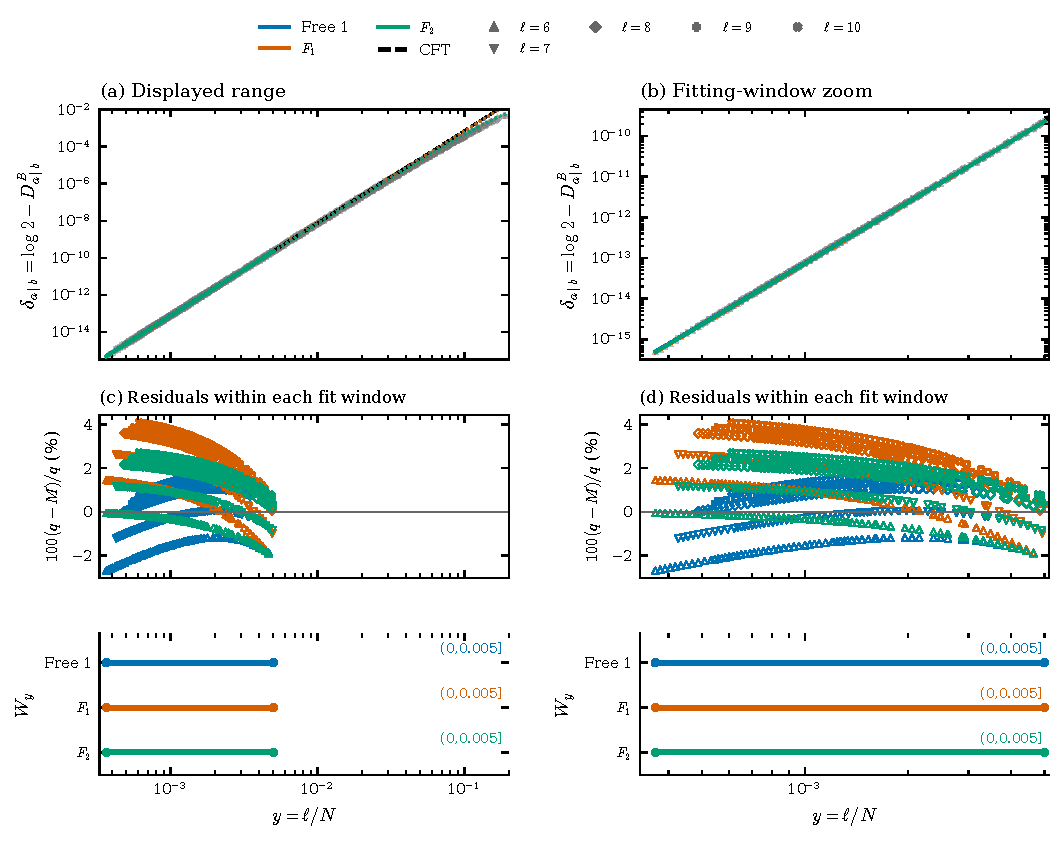
\includegraphics[width=.94\linewidth]{../figs/pair_large_boson_00_3s_s.pdf}\par\smallskip
\begingroup\scriptsize\setlength{\tabcolsep}{4pt}
\begin{tabular}{lllrrrrr}\toprule
Set & Model & $W_z$ & $m$ & $c_0$ & $r^{(0)}$ & $c_1$ & $r^{(1)}$\\\midrule
Both & Free 1 & $(0,0.005]$ & 317 & 66.924 & 4.9836496 & --- & ---\\
Both & $F_1$ & $(0,0.005]$ & 317 & 73.093 & 5 & --- & ---\\
Both & $F_2$ & $(0,0.005]$ & 317 & 74.307 & 5 & -265.58 & 6\\
\midrule
Both & CFT & --- & --- & 75.109 & 5 & --- & ---\\
\bottomrule\end{tabular}
\endgroup
\caption{Compact boson, large intervals, $00\mid 3s,s$, at $p=1/2$, $\ell=6,\ldots,10$, and the complete size grid in Eq.~\eqref{eq:extended-grid}. Here $z=y$ and $q=\delta=\log2-D^B$. Left: all computed data through $z=0.20$; right: a zoom into the common fitting window. Both columns show the same Free 1, $F_1$, and $F_2$ fits. All six directions of this CFT and interval type use the same window. Gray markers denote the data. Colored solid segments lie inside each model\textquotesingle s fitting interval; dotted segments are extrapolations. Black dashed is the analytical CFT leading deficit. The observable axes are logarithmic and span the measured data; nonpositive predictions cannot appear there and out-of-range extrapolations leave the panel. Residual ordinates are linear and show $100(q-M)/q$ only on each model\textquotesingle s fitted observations. Bars give the exact fitting intervals. The parameter block follows Eq.~\eqref{eq:fit}, with $c_0,c_1$ multiplying $z^{r^{(0)}},z^{r^{(1)}}$; all coefficients include powers of $\pi$. A dash means an absent fitted term, or no fitting window for CFT. Values shown are rounded; curves use full precision.}
\label{fig:pair-large_boson-00-3s_s}
\end{figure}
\begin{figure}[!htbp]\centering
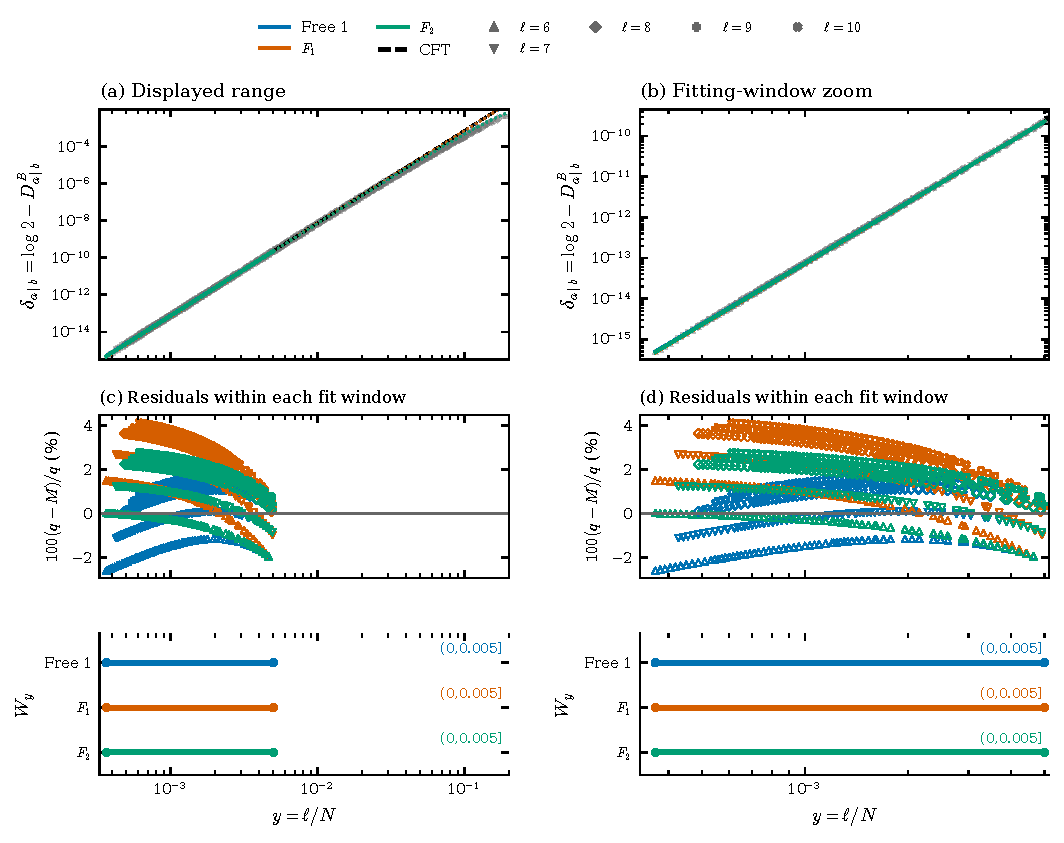
\includegraphics[width=.94\linewidth]{../figs/pair_large_boson_3s_s_00.pdf}\par\smallskip
\begingroup\scriptsize\setlength{\tabcolsep}{4pt}
\begin{tabular}{lllrrrrr}\toprule
Set & Model & $W_z$ & $m$ & $c_0$ & $r^{(0)}$ & $c_1$ & $r^{(1)}$\\\midrule
Both & Free 1 & $(0,0.005]$ & 317 & 66.96 & 4.9838386 & --- & ---\\
Both & $F_1$ & $(0,0.005]$ & 317 & 73.058 & 5 & --- & ---\\
Both & $F_2$ & $(0,0.005]$ & 317 & 74.252 & 5 & -261.18 & 6\\
\midrule
Both & CFT & --- & --- & 75.109 & 5 & --- & ---\\
\bottomrule\end{tabular}
\endgroup
\caption{Compact boson, large intervals, $3s,s\mid 00$, at $p=1/2$, $\ell=6,\ldots,10$, and the complete size grid in Eq.~\eqref{eq:extended-grid}. Here $z=y$ and $q=\delta=\log2-D^B$. Left: all computed data through $z=0.20$; right: a zoom into the common fitting window. Both columns show the same Free 1, $F_1$, and $F_2$ fits. All six directions of this CFT and interval type use the same window. Gray markers denote the data. Colored solid segments lie inside each model\textquotesingle s fitting interval; dotted segments are extrapolations. Black dashed is the analytical CFT leading deficit. The observable axes are logarithmic and span the measured data; nonpositive predictions cannot appear there and out-of-range extrapolations leave the panel. Residual ordinates are linear and show $100(q-M)/q$ only on each model\textquotesingle s fitted observations. Bars give the exact fitting intervals. The parameter block follows Eq.~\eqref{eq:fit}, with $c_0,c_1$ multiplying $z^{r^{(0)}},z^{r^{(1)}}$; all coefficients include powers of $\pi$. A dash means an absent fitted term, or no fitting window for CFT. Values shown are rounded; curves use full precision.}
\label{fig:pair-large_boson-3s_s-00}
\end{figure}
\begin{figure}[!htbp]\centering
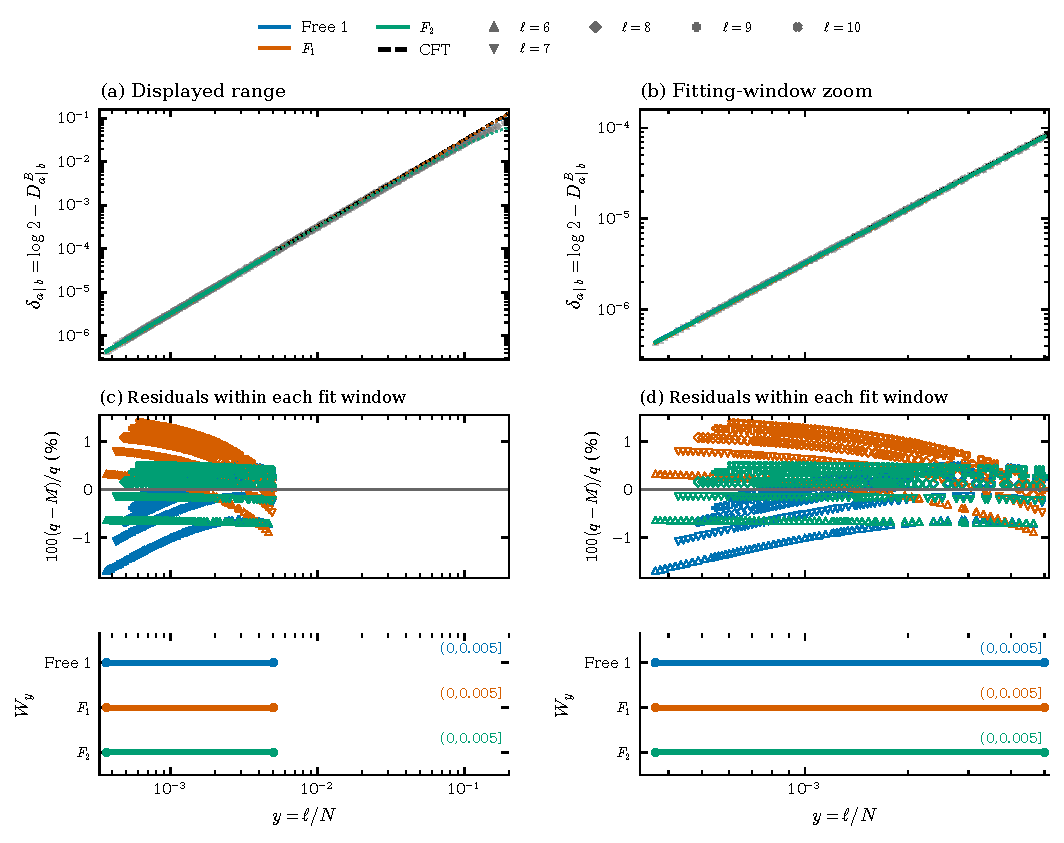
\includegraphics[width=.94\linewidth]{../figs/pair_large_boson_ss_3s_s.pdf}\par\smallskip
\begingroup\scriptsize\setlength{\tabcolsep}{4pt}
\begin{tabular}{lllrrrrr}\toprule
Set & Model & $W_z$ & $m$ & $c_0$ & $r^{(0)}$ & $c_1$ & $r^{(1)}$\\\midrule
Both & Free 1 & $(0,0.005]$ & 317 & 3.069 & 1.9914473 & --- & ---\\
Both & $F_1$ & $(0,0.005]$ & 317 & 3.2185 & 2 & --- & ---\\
Both & $F_2$ & $(0,0.005]$ & 317 & 3.2529 & 2 & -8.6617 & 3\\
\midrule
Both & CFT & --- & --- & 3.2899 & 2 & --- & ---\\
\bottomrule\end{tabular}
\endgroup
\caption{Compact boson, large intervals, $ss\mid 3s,s$, at $p=1/2$, $\ell=6,\ldots,10$, and the complete size grid in Eq.~\eqref{eq:extended-grid}. Here $z=y$ and $q=\delta=\log2-D^B$. Left: all computed data through $z=0.20$; right: a zoom into the common fitting window. Both columns show the same Free 1, $F_1$, and $F_2$ fits. All six directions of this CFT and interval type use the same window. Gray markers denote the data. Colored solid segments lie inside each model\textquotesingle s fitting interval; dotted segments are extrapolations. Black dashed is the analytical CFT leading deficit. The observable axes are logarithmic and span the measured data; nonpositive predictions cannot appear there and out-of-range extrapolations leave the panel. Residual ordinates are linear and show $100(q-M)/q$ only on each model\textquotesingle s fitted observations. Bars give the exact fitting intervals. The parameter block follows Eq.~\eqref{eq:fit}, with $c_0,c_1$ multiplying $z^{r^{(0)}},z^{r^{(1)}}$; all coefficients include powers of $\pi$. A dash means an absent fitted term, or no fitting window for CFT. Values shown are rounded; curves use full precision.}
\label{fig:pair-large_boson-ss-3s_s}
\end{figure}
\begin{figure}[!htbp]\centering
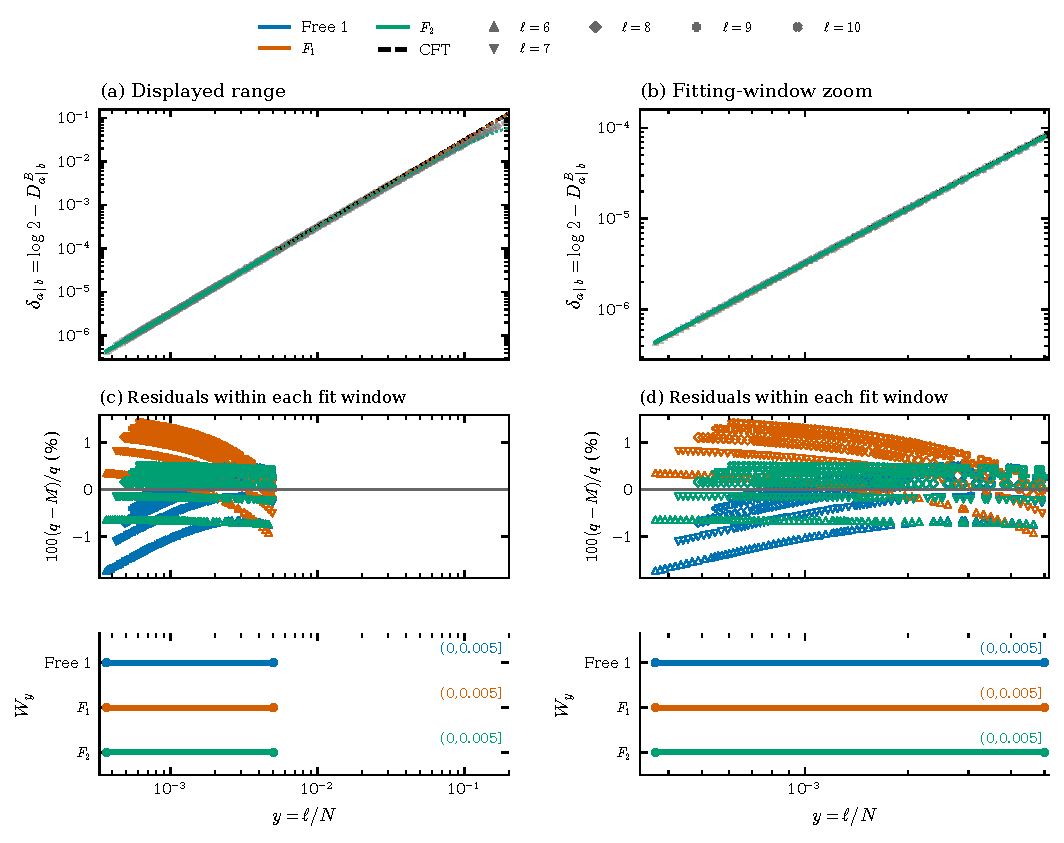
\includegraphics[width=.94\linewidth]{../figs/pair_large_boson_3s_s_ss.pdf}\par\smallskip
\begingroup\scriptsize\setlength{\tabcolsep}{4pt}
\begin{tabular}{lllrrrrr}\toprule
Set & Model & $W_z$ & $m$ & $c_0$ & $r^{(0)}$ & $c_1$ & $r^{(1)}$\\\midrule
Both & Free 1 & $(0,0.005]$ & 317 & 3.0643 & 1.9912306 & --- & ---\\
Both & $F_1$ & $(0,0.005]$ & 317 & 3.2176 & 2 & --- & ---\\
Both & $F_2$ & $(0,0.005]$ & 317 & 3.2528 & 2 & -8.8758 & 3\\
\midrule
Both & CFT & --- & --- & 3.2899 & 2 & --- & ---\\
\bottomrule\end{tabular}
\endgroup
\caption{Compact boson, large intervals, $3s,s\mid ss$, at $p=1/2$, $\ell=6,\ldots,10$, and the complete size grid in Eq.~\eqref{eq:extended-grid}. Here $z=y$ and $q=\delta=\log2-D^B$. Left: all computed data through $z=0.20$; right: a zoom into the common fitting window. Both columns show the same Free 1, $F_1$, and $F_2$ fits. All six directions of this CFT and interval type use the same window. Gray markers denote the data. Colored solid segments lie inside each model\textquotesingle s fitting interval; dotted segments are extrapolations. Black dashed is the analytical CFT leading deficit. The observable axes are logarithmic and span the measured data; nonpositive predictions cannot appear there and out-of-range extrapolations leave the panel. Residual ordinates are linear and show $100(q-M)/q$ only on each model\textquotesingle s fitted observations. Bars give the exact fitting intervals. The parameter block follows Eq.~\eqref{eq:fit}, with $c_0,c_1$ multiplying $z^{r^{(0)}},z^{r^{(1)}}$; all coefficients include powers of $\pi$. A dash means an absent fitted term, or no fitting window for CFT. Values shown are rounded; curves use full precision.}
\label{fig:pair-large_boson-3s_s-ss}
\end{figure}
